% !TEX TS-program = xelatex
% !TEX encoding = UTF-8

% This is a simple template for a XeLaTeX document using the "article" class,
% with the fontspec package to easily select fonts.

\documentclass[11pt]{report} % use larger type; default would be 10pt
\usepackage{fontspec} % Font selection for XeLaTeX; see fontspec.pdf for documentation
\defaultfontfeatures{Mapping=tex-text} % to support TeX conventions like ``---''
\usepackage{xunicode} % Unicode support for LaTeX character names (accents, European chars, etc)
\usepackage{xltxtra} % Extra customizations for XeLaTeX
% \fontspec{"[DroidSerif.ttf]"}
% \setmainfont{Droid Serif} % set the main body font (\textrm), assumes Charis SIL is installed
%\setsansfont{Deja Vu Sans}
%\setmonofont{Deja Vu Mono}
\usepackage{amsmath}
\usepackage{xfrac,unicode-math}
\usepackage{siunitx}
\setmathfont[version=cambria]{Cambria Math}
\mathversion{cambria}
\usepackage{cleveref}
% other LaTeX packages.....
\usepackage{geometry} % See geometry.pdf to learn the layout options. There are lots.
\geometry{letterpaper} % or letterpaper (US) or a5paper or....
%\usepackage[parfill]{parskip} % Activate to begin paragraphs with an empty line rather than an indent

\usepackage{graphicx} % support the \includegraphics command and options

\title{237D Fusion Technology \\
Introduction to Solid Breeder}
\author{Jon Van Lew}
%\date{} % Activate to display a given date or no date (if empty),
         % otherwise the current date is printed 


\begin{document}
\maketitle
Key Concepts
\begin{enumerate}
\item{Use of a lithiated ceramic must have:}
\begin{itemize}
\item{high melting temperature}
\item{desirable neutronics and irradiation characteristics (no bad transmutation nuclides)}
\item{chemical stability \& compatibility with structural material}
\item{sufficiently high T release rates}
\item{high Li density}
\item{open porosity for purging T}
\end{itemize}
\item{Always separately cooled with (with \textit{e.g.} helium or water)}
\item{Necessity of neutron multiplication}
\item{Surrounded by a structure of reduced-activation ferritic steel}
\end{enumerate}


Disadvantages of lithium
\begin{itemize}
\item {It is chemically active meaning safety is an issue. As an example, here are two reactions with oxygen along with their heats of formation
\begin{align*}
2\mathrm{Li} + \frac{1}{2}\mathrm{O} &\rightarrow \mathrm{Li}_2\mathrm{O} - 142.75~\text{kCal/mol}\\
2\mathrm{Li} + \mathrm{O} &\rightarrow \mathrm{Li}_2\mathrm{O}_2 - 151.9~\text{kCal/mol}
\end{align*}
note: a negative heat of formation means an exothermic reaction. Lithium will exothermically react with water (or air, concrete, or any moisture-containing materials) with high amounts of energy released. Of primary concern in lithium fires is the peak flame temperature. This will determine, to a large extent, whether many radioactive species become air-borne by vaporization. The flame temperature depends on many variables. Some investigations found it to be  about 2500 K which would cause some materials to melt but not vaporize.}
\item MHD effects -- liquid metals have high electrical conductivity. In a magnetic field this leads to a $\vec{J}\times\vec{B}$ force. This in turn leads to pressure drops in the magnetic fluid. To overcome the pressure drop requires increased pressurization and pumping power. The increase in pressurization leads to an increase in stresses of the containing structures and pumping power means more leeching of power from the reactor power plant.
\item Liquid metals tend to be corrosive. Corrosion products transport from radioactive structural materials and are carried downstream into sensitive regions.
\end{itemize}

\subsection{Lithium}
Review lithium reactions...
\begin{align}
\mathrm{n} + ~^7\mathrm{Li} &\xrightarrow ~\mathrm{n}+\alpha + \mathrm{T} -2.47~\text{MeV}\label{eq:Li7T}\\
\mathrm{n} + ~^6\mathrm{Li} &\xrightarrow ~ \alpha + \mathrm{T} +4.78~\text{MeV} \label{eq:Li6T}
\end{align}

\begin{figure}
\centering
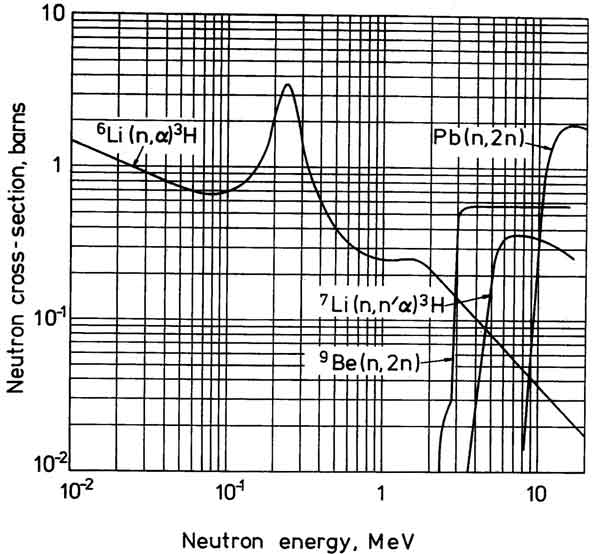
\includegraphics[width=0.8\textwidth]{../images/breeding_xsecs} 
\caption{Cross-sections of various blanket materials. Note the threshold for the $^7$Li and neutron multiplying reactions.}
\label{fig:xsects}
\end{figure}

Natural lithium occurs with the isotopic abundances of 92.58\% for $^7Li$ and 7.42\% for $^6Li$. Lithium metal is soft, has a low density (of 0.53 g/cm$^3$), and has a physical appearance similar to lead. The average abundance of lithium in the Earth's crust is approximately 65 parts per million by weight. The concentration of lithium in sea water is also about 0.17 g/m$^3$. Lithium reserves are estimated to be sufficient for the United States' electrical demand for more than 600 years.

Mean-free-path of tritium-producing reaction in natural lithium
\begin{align*}
\lambda_t & > \SI{70}{\centi\meter} && n(\SI{14}{\mega\electronvolt})\\
\lambda_t & \approx \SI{2}{\centi\meter} && n(\SI{1}{\electronvolt}) 
\end{align*}

In 90\% enriched lithium-6,
\begin{align*}
\lambda_t & \approx \SI{0.15}{\centi\meter} && n(\SI{1}{\electronvolt}) 
\end{align*}
lithium-6 cross-section at \SI{0.025}{\electronvolt} is %\SI{740}{\barns}.

Intentionally shifting to softer neutron energy spectrum to shorten mean-free-path will preclude the lithium-7 reaction.

Inelastic scattering of other materials with drop neutrons below lithium-7 threshold.

Must have neutron multiplier


\section{Neutron multiplication in solid breeder}
(n,2n) reactions are always endothermic and therefore always have threshold energies

(n,2n) help raise tritium breeding ratio and increase neutrons for energy multiplication

The two most prominently analyzed neutron multipliers for a fusion reactor are beryllium and lead. Beryllium has a very high nuclide density while also being very light, with a high melting temperature, and high thermal conductivity. However it undergoes a 2-$\alpha$ reaction that causes trapped helium to swell the material. There is also a rarely occurring reaction with beryllium that generates tritium; it is frequent enough to cause a concern with contamination.

\begin{align}
\mathrm{n} + ~^9_4\mathrm{Be} &\xrightarrow ~2\mathrm{n}+2\alpha + \mathrm{T} -1.57~\text{MeV}\label{eq:Be-n}
\end{align}

melting temperature of beryllium is \SI{1250}{\celsius}, melting temperature of lead is \SI{327}{\celsius}. Thermal energy of Be is 1.7 MeV, Pb is 7 MeV. Choose beryllium for non-mobile breeder.

Chemical composition of beryllium,
\begin{itemize}
\item{BeO}
\begin{itemize}
\item{excellent compatibility with structural steel}
\item{carciongen, causes beryllium disease if inhaled}
\end{itemize}
\item{Be}
\begin{itemize}
\item{incompatibility with strucuture steel, forming FeBe13}
\item{Be reaction with water forming BeO (Be + H2O -> BeO + H2)}
\item{2Be + O2 -> 2BeO}
\end{itemize}
\item{Be12Ti}
\begin{itemize}
\item{compatible with ss.}
\item{high metling temperature}
\item{less swelling than Be}
\item{higher chemical stability}
\item{high Be density maintains neutron multiplication characteristics}
\end{itemize}
\end{itemize}
Bear in mind limited Be abundancy on Earth. (remember Homework set)

Beryllium will also exist as a pebble bed. The following reaction has small probability of occurance (check cross-section for this reaction)
\begin{align}
\mathrm{n} + ~^9_4\mathrm{Be} &\xrightarrow ~ ^4_2\mathrm{He} + ~^6_2\mathrm{He}\\
~^6_2\mathrm{He} &\xrightarrow ~ ^6_3\mathrm{Li} + \beta^-\\
\mathrm{n} + ~^6_3\mathrm{Li} &\xrightarrow ~ T + \alpha
\end{align}

Diffusional release of T from irradiated beryllium is very slow, measured in BeO to be about \num{1e-15} cm2/sec at 900C. The diffusional path should be kept aroudn 1 micron for T inventory concerns.

\section{Lithium ceramic}
Li2O, only ceramic that could possible achieve TBR>1 without dedicated neutron multiplier. Highly hygroscopic.
Li2O + H2O -> 2LiOH deltaH = 128.9 kJ/mol
LiOH is highly corrosive

Li2TiO3 has acceptable Li density, not hygroscopic, has lower activation, similar T release to lithium zirconate. Mechanically stronger than Li4SiO4.

Li4SiO4 has weak crush strength, acceptable Li density, stable (can't read my notes)


Pebble form chosen for open porosity, large surface area to volume, maintain wall contact. But note that pebble bed is not the only solution. It is a good choice to satisfy the design requirements but pebble beds make a low conductivity material even worse at thermal transport.

Nevertheless, focusing on pebble bed form... specific performance requirements...

Tritium release, a function of grain size, microsctructure, open/closed porosity. The material integrity is a functino of pebble size distribution, sphericity, mechanical strength, chemical stability.


Common features of pebble bed designs...

low pressure, slow mass flow rate helium purge gas to extract T. High pressure coolant in structure. Permissible temperature window of Li bed. All heat removal via conduction to walls (through contacts and helium).

\subsection{Purge gas}
Purge - keep delta-P around 0.01 MPa. mdot = 0.1 to 0.3 g/s.

Review pressure drop correlations.

\subsection{Coolant}

Example values: coolant - P = 8 MPa. Tin = 300 C, Tout = 500 C (kept below 600 C for structural integrity of container).

Nothing exotic. standard heat transfer of a fluid in a duct. Must consider safety issues of high pressure coolant.

\subsection{Pebble bed}
(Discuss how its treated as a continuum, etc.)
\end{document}